% \documentclass[convert={density=300,size=1080x800,outext=.png}]{standalone}
% \documentclass[convert={density=300,outext=.png}]{standalone}
\documentclass[convert={density=175,outext=.png}]{standalone}

\usepackage{tikz}
\usetikzlibrary{matrix,arrows}

\begin{document}

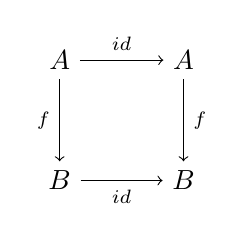
\begin{tikzpicture}[descr/.style={fill=white,inner sep=2.5pt}]
\matrix (m) [matrix of math nodes, row sep=3em, column sep=3em]
{ A & A \\
  B & B \\ };
\path[->,font=\scriptsize]
(m-1-1) edge node[auto]      {$ id $}       (m-1-2)
(m-1-1) edge node[auto,swap] {$ f $}        (m-2-1)
(m-1-2) edge node[auto]      {$ f $}        (m-2-2)
(m-2-1) edge node[auto,swap] {$ id $}       (m-2-2);
\end{tikzpicture}

\end{document}
